\documentclass[10pt,t]{beamer}


%\setbeamersize{text margin left=10pt,text margin right=10pt}
\usetheme{lehigh}

\usefonttheme{professionalfonts}
\usefonttheme{serif}

\pgfdeclarelayer{background}
\pgfdeclarelayer{foreground}
\pgfsetlayers{background,main,foreground}

% add packages to use
%\usepackage[latin1]{inputenc}
%\usepackage[english]{babel}
%\usepackage[normalem]{ulem}
\usepackage{times}
\usepackage[T1]{fontenc}
\usepackage{pgf,pgfarrows,pgfnodes,pgfautomata,pgfheaps,pgfshade}
\usepackage{amsmath,amssymb,amsfonts,subfigure,pifont}
\usepackage{graphicx}
\usepackage{multirow,multicol}
\usepackage{tabularx}
\usepackage{booktabs}
\usepackage{colortbl}
\usepackage{fancyvrb,listings}
\usepackage{algorithm,algpseudocode}
%\usepackage{keystroke}
\usepackage{etex}
\usepackage{hyperref}
\usepackage{tikz}
\usetikzlibrary{trees,matrix,shapes,arrows}
\usetikzlibrary{calc}



% The following color are for listing environment 
\definecolor{dkgreen}{rgb}{0,0.6,0}
\definecolor{DarkGreen}{rgb}{0.0,0.3,0.0}
\definecolor{gray}{rgb}{0.5,0.5,0.5}
\definecolor{mauve}{rgb}{0.58,0,0.82}
\definecolor{Blue}{rgb}{0.0,0.0,0.8} 
\definecolor{dodgerblue}{rgb}{0.1,0.1,1.0}
\definecolor{indigo}{rgb}{0.41,0.1,0.0}
\definecolor{seagreen}{rgb}{0.1,1.0,0.1}


\lstset{%
language=bash,                % the language of the code
basicstyle=\tiny\ttfamily,           % the size of the fonts that are used for the code
showspaces=false,               % show spaces adding particular underscores
showstringspaces=false,         % underline spaces within strings
showtabs=false,                 % show tabs within strings adding particular underscores
%frame=single,                   % adds a frame around the code
%rulecolor=\color{black},        % if not set, the frame-color may be changed on line-breaks within not-black text (e.g. comments (green here))
tabsize=2,                      % sets default tabsize to 2 spaces
%captionpos=b,                   % sets the caption-position to bottom
breaklines=true,                % sets automatic line breaking
breakatwhitespace=false,        % sets if automatic breaks should only happen at whitespace
%title=\lstname,                   % show the filename of files included with \lstinputlisting;
% also try caption instead of title
keywordstyle=\color{blue},          % keyword style
commentstyle=\color{dkgreen},       % comment style
stringstyle=\color{mauve},         % string literal style
escapeinside={!}{!},            % if you want to add LaTeX within your code
morekeywords={*,\dots,elif},              % if you want to add more keywords to the set
deletekeywords={\dots},              % if you want to delete keywords from the given language
%morecomment=[l]{//}
}
\lstset{%
language=csh,                % the language of the code
basicstyle=\tiny\ttfamily,           % the size of the fonts that are used for the code
showspaces=false,               % show spaces adding particular underscores
showstringspaces=false,         % underline spaces within strings
showtabs=false,                 % show tabs within strings adding particular underscores
%frame=single,                   % adds a frame around the code
%rulecolor=\color{black},        % if not set, the frame-color may be changed on line-breaks within not-black text (e.g. comments (green here))
tabsize=2,                      % sets default tabsize to 2 spaces
captionpos=b,                   % sets the caption-position to bottom
breaklines=true,                % sets automatic line breaking
breakatwhitespace=false,        % sets if automatic breaks should only happen at whitespace
%title=\lstname,                   % show the filename of files included with \lstinputlisting;
% also try caption instead of title
keywordstyle=\color{blue},          % keyword style
commentstyle=\color{dkgreen},       % comment style
stringstyle=\color{mauve},         % string literal style
escapeinside={\%*}{*)},            % if you want to add LaTeX within your code
morekeywords={*,\dots,elif},              % if you want to add more keywords to the set
deletekeywords={\dots},              % if you want to delete keywords from the given language
%morecomment=[l]{//}
}

\lstdefinestyle{LINUX}
{
    backgroundcolor=\color{white},
    basicstyle=\tiny\ttfamily,
    keywordstyle=\color{blue},
    morekeywords={apacheco,Tutorials,BASH,scripts,day1,examples},
    literate={>}{{\textcolor{blue}{>}}}1
         {/}{{\textcolor{blue}{/}}}1
         {./}{{\textcolor{black}{./ }}}1
         {~}{{\textcolor{blue}{\textasciitilde}}}1,
}

\lstdefinestyle{customc}{
  belowcaptionskip=1\baselineskip,
  breaklines=true,
  xleftmargin=\parindent,
  language=C,
  showstringspaces=false,
  basicstyle=\tiny\ttfamily,
  keywordstyle=\bfseries\color{green!40!black},
  commentstyle=\upshape\color{red!90!white},
  identifierstyle=\color{blue},
  stringstyle=\color{orange},
}
\lstdefinelanguage{OmpFortran}[]{Fortran}{
   rulesepcolor=\color{black},
   %
   extendedchars=true,
   %
   morecomment=[l] [\bfseries\color{red!90!white}]{!\$omp},
   morecomment=[l] [\bfseries\color{red!90!white}]{c\$omp},
   morecomment=[l] [\bfseries\color{red!90!white}]{*\$omp},
   morecomment=[l] [\bfseries\color{red!90!white}]{!\$acc},
   morecomment=[l] [\bfseries\color{red!90!white}]{c\$acc},
   morecomment=[l] [\bfseries\color{red!90!white}]{*\$acc},
}[comments]

\lstdefinelanguage{OmpC}[]{OmpFortran}{
   rulesepcolor=\color{black},
   %
   extendedchars=true,
   %
   morecomment=[l] [\bfseries\color{red!90!white}]{\#pragma\ omp},
   morecomment=[l] [\bfseries\color{red!90!white}]{\#pragma\ acc},
}[comments]

\lstset{escapechar=@,style=customc}
\lstset{literate=%
   *{0}{{{\color{blue}0}}}1
    {1}{{{\color{blue}1}}}1
    {2}{{{\color{blue}2}}}1
    {3}{{{\color{blue}3}}}1
    {4}{{{\color{blue}4}}}1
    {5}{{{\color{blue}5}}}1
    {6}{{{\color{blue}6}}}1
    {7}{{{\color{blue}7}}}1
    {8}{{{\color{blue}8}}}1
    {9}{{{\color{blue}9}}}1
}

\algrenewcommand\algorithmicfunction{\textbf{program}}
\algblockdefx[Program]{Program}{EndProgram}[1]{\textbf{program} \textsc{#1}}[1]{\textbf{end program} \textsc{#1}}
\algloopdefx[doloop]{Do}[1]{\textbf{do} #1}
\algcblockdefx[doloop]{If}{Do}{EndDo}
[1]{\textbf{do} #1}{\textbf{end do}}


\DeclareSymbolFont{extraup}{U}{zavm}{m}{n}
%\DeclareMathSymbol{\vardiamond}{\mathalpha}{extraup}{87}
\newcommand{\cmark}{\ding{51}}
\newcommand{\xmark}{\ding{55}}
\newcommand{\smark}{\ding{77}}
\newcommand*\vardiamond{\textcolor{lubrown}{%
  \ensuremath{\blacklozenge}}}
\newcommand*\mybigstar{\textcolor{lubrown!90!yellow}{%
  \ensuremath{\bigstar}}}
\newcommand*\up{\textcolor{green!80!black}{%
  \ensuremath{\blacktriangle}}}
\newcommand*\down{\textcolor{red}{%
  \ensuremath{\blacktriangledown}}}
\newcommand*\const{\textcolor{darkgray}%
  {\textbf{--}}}
\newcommand*\enter{\tikz[baseline=-0.5ex] \draw[<-] (0,0) -| (0.5,0.1);}
\newcommand{\bftt}[1]{\textbf{\texttt{#1}}}
\newcommand{\bflub}[1]{\textbf{\color{lubrown}#1}}
\newcommand{\lstfortran}[1]{\lstinline[language={[90]Fortran},basicstyle=\small\ttfamily]|#1|}
\newcommand{\lstC}[1]{\lstinline[language=C,basicstyle=\small\ttfamily]|#1|}
\newcommand{\Verblubrown}[1]{\Verb[formatcom=\color{lubrown},fontseries=b,commandchars=\\\{\}]|#1|}
\newcommand{\Verblue}[1]{\Verb[formatcom=\color{lublue},fontseries=b,commandchars=\\\{\}]!#1!}
\newcommand{\Verbblue}[2][b]{\Verb[formatcom=\color{lublue},fontshape=#1,commandchars=\\\{\}]|#2|}
\newcommand{\Verblubrownp}[1]{\Verb[formatcom=\color{lubrown},fontseries=b,commandchars=\\\{\}]!#1!}
\newcommand{\Verbred}[1]{\Verb[formatcom=\color{red},commandchars=\\\{\}]|#1|}
\newcommand{\Verbindigo}[1]{\Verb[formatcom=\color{indigo},fontsize=\fontsize{7.5}{8}\selectfont,commandchars=\\\{\}]!#1!}

\newcolumntype{a}{>{\columncolor{lulime}}c}
\newcolumntype{b}{>{\columncolor{lulime!50}}c}
\newcolumntype{d}{>{\columncolor{lulime!40}}c}
\newcolumntype{e}{>{\columncolor{lulime}}l}
\newcolumntype{f}{>{\columncolor{lulime!50}}l}

                           
% LOGOS
\pgfdeclareimage[height=0.55cm]{lucolor-logo}{LehighU_official-logo_Color.png}
\rplogo{\pgfuseimage{lucolor-logo}}
\pgfdeclareimage[height=0.55cm]{luwhite-logo}{LehighU_official-logo_White.png}
\tplogo{\pgfuseimage{luwhite-logo}}
% footer logo
%\pgfdeclareimage[width=0.3\paperwidth]{university-logo}{lulogo}
%\tllogo{\pgfuseimage{university-logo}}

%titlepage logo
%\titlegraphic{
\includegraphics[scale=0.5]{lu}}

\beamertemplateballitem


\beamertemplateballitem

\title{Parallel Programming Concepts}
\subtitle{}
\author{Alexander B. Pacheco}
\institute{\href{http://researchcomputing.lehigh.edu}{LTS Research Computing}}
%\date{\today}

% Delete this, if you do not want the table of contents to pop up at
% the beginning of each subsection:
\AtBeginSection[]
{
  \begingroup
  \setbeamertemplate{background canvas}[vertical shading][bottom=lubrown,top=lubrown]
  \setbeamertemplate{footline}[myfootline] 
  \setbeamertemplate{section page}[mysection]
  \frame[c]{
    \sectionpage
  }
  \endgroup
}


\begin{document}

\begin{frame}
  \titlepage
\end{frame}

\begin{frame}[c]{Outline}
  \tableofcontents
\end{frame}

\section{Introduction}
\begin{frame}
  \frametitle{What is Serial Computing?}
  \begin{itemize}
  \item Traditionally, software has been written for serial computation:
    \begin{itemize}
    \item A problem is broken into a discrete series of instructions
    \item Instructions are executed sequentially one after another
    \item Executed on a single processor
    \item Only one instruction may execute at any moment in time
    \end{itemize}
  \end{itemize}
  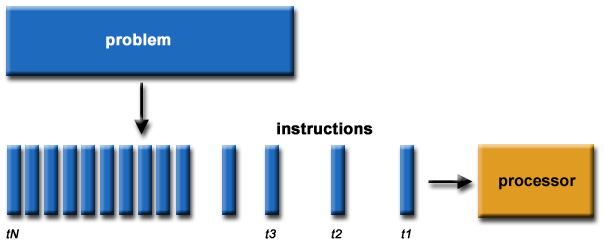
\includegraphics[width=\textwidth]{./serialProblem}
\end{frame}

\begin{frame}
  \frametitle{What is Parallel Computing?}
  \begin{itemize}
  \item In the simplest sense, parallel computing is the simultaneous use of multiple compute resources to solve a computational problem:
    \begin{itemize}
    \item A problem is broken into discrete parts that can be solved concurrently
    \item Each part is further broken down to a series of instructions
    \item Instructions from each part execute simultaneously on different processors
    \item An overall control/coordination mechanism is employed
    \item The computational problem should be able to:
      \begin{itemize}
      \item Be broken apart into discrete pieces of work that can be solved simultaneously;
      \item Execute multiple program instructions at any moment in time;
      \item Be solved in less time with multiple compute resources than with a single compute resource.
      \end{itemize}
    \item The compute resources are typically:
      \begin{itemize}
      \item A single computer with multiple processors/cores
      \item An arbitrary number of such computers connected by a network
      \end{itemize}
    \end{itemize}
  \end{itemize}
\end{frame}

\begin{frame}
  \frametitle{Why Parallel Computing?}
  \begin{itemize}
  \item Parallel computing might be the only way to achieve certain goals
    \begin{itemize}
    \item Problem size (memory, disk etc.)
    \item Time needed to solve problems
    \end{itemize}
  \item Parallel computing allows us to take advantage of ever-growing parallelism at all levels
    \begin{itemize}
    \item  Multi-core, many-core, cluster, grid, cloud, $\cdots$
    \end{itemize}
  \end{itemize}
  \begin{center}
    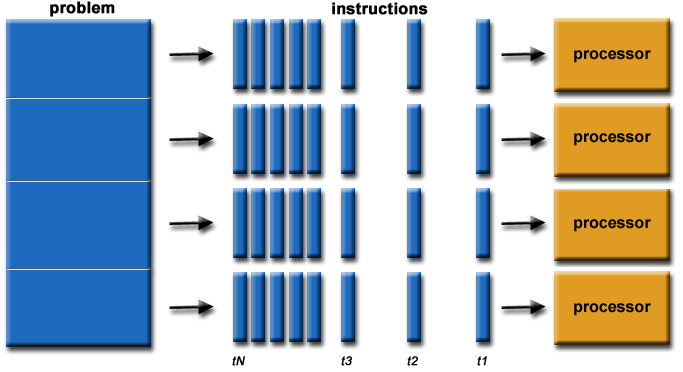
\includegraphics[width=0.7\textwidth]{./parallelProblem}
  \end{center}
\end{frame}

\begin{frame}
  \frametitle{What are Parallel Computers?}
  \begin{itemize}
  \item Virtually all stand-alone computers today are parallel from a hardware perspective:
    \begin{itemize}
    \item Multiple functional units (L1 cache, L2 cache, branch, prefetch, decode, floating-point, graphics processing (GPU), integer, etc.)
    \item Multiple execution units/cores
    \item Multiple hardware threads
    \item Networks connect multiple stand-alone computers (nodes) to make larger parallel computer clusters.
    \end{itemize}
  \end{itemize}
\end{frame}

\begin{frame}[allowframebreaks,c]
  \frametitle{Why Use Parallel Computing?}
  \begin{itemize}
  \item The Real World is Massively Parallel:
    \begin{itemize}
    \item In the natural world, many complex, interrelated events are happening at the same time, yet within a temporal sequence.
    \item Compared to serial computing, parallel computing is much better suited for modeling, simulating and understanding complex, real world phenomena.
    \end{itemize}
    \begin{center}
      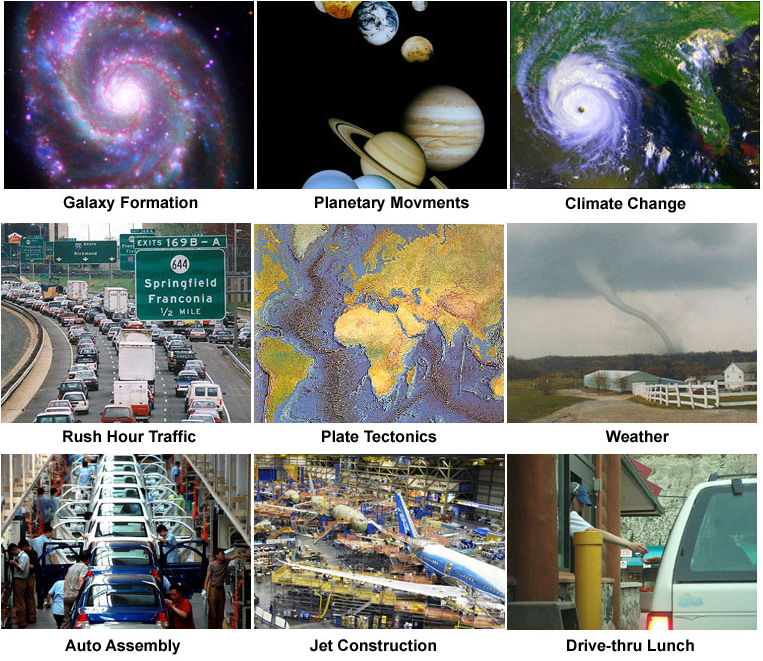
\includegraphics[width=0.5\textwidth]{./realworldcollage}
    \end{center}
    \framebreak
  \item SAVE TIME AND/OR MONEY:
    \begin{itemize}
    \item In theory, throwing more resources at a task will shorten its time to completion, with potential cost savings.
    \item Parallel computers can be built from cheap, commodity components.
    \end{itemize}
    %\framebreak
  \item SOLVE LARGER / MORE COMPLEX PROBLEMS:
    \begin{itemize}
    \item Many problems are so large and/or complex that it is impractical or impossible to solve them on a single computer, especially given limited computer memory.
    \item Example: "Grand Challenge Problems" (en.wikipedia.org/wiki/Grand\_Challenge) requiring PetaFLOPS and PetaBytes of computing resources.
    \item Example: Web search engines/databases processing millions of transactions every second
    \end{itemize}
    %\framebreak
  \item PROVIDE CONCURRENCY:
    \begin{itemize}
    \item A single compute resource can only do one thing at a time. Multiple compute resources can do many things simultaneously.
    \item Example: Collaborative Networks provide a global venue where people from around the world can meet and conduct work "virtually".
    \end{itemize}
    \framebreak
  \item TAKE ADVANTAGE OF NON-LOCAL RESOURCES:
    \begin{itemize}
    \item Using compute resources on a wide area network, or even the Internet when local compute resources are scarce or insufficient.
    \item Example: SETI@home (setiathome.berkeley.edu) over 1.5 million users in nearly every country in the world. Source: www.boincsynergy.com/stats/ (June, 2015).
    \item Example: Folding@home (folding.stanford.edu) uses over 160,000 computers globally (June, 2015)
    \end{itemize}
    %\framebreak
  \item MAKE BETTER USE OF UNDERLYING PARALLEL HARDWARE:
    \begin{itemize}
    \item Modern computers, even laptops, are parallel in architecture with multiple processors/cores.
    \item Parallel software is specifically intended for parallel hardware with multiple cores, threads, etc.
    \item In most cases, serial programs run on modern computers "waste" potential computing power.
    \end{itemize}
    \framebreak
  \item The Future:
    \begin{columns}[c]
      \column{0.5\textwidth}
      \begin{itemize}
      \item During the past 20+ years, the trends indicated by ever faster networks, distributed systems, and multi-processor computer architectures (even at the desktop level) clearly show that parallelism is the future of computing.
      \item In this same time period, there has been a greater than 500,000x increase in supercomputer performance, with no end currently in sight.
      \item The race is already on for Exascale Computing!
      \item[] Exaflop = $10^{18}$ calculations per second
      \end{itemize}
      \column{0.5\textwidth}
      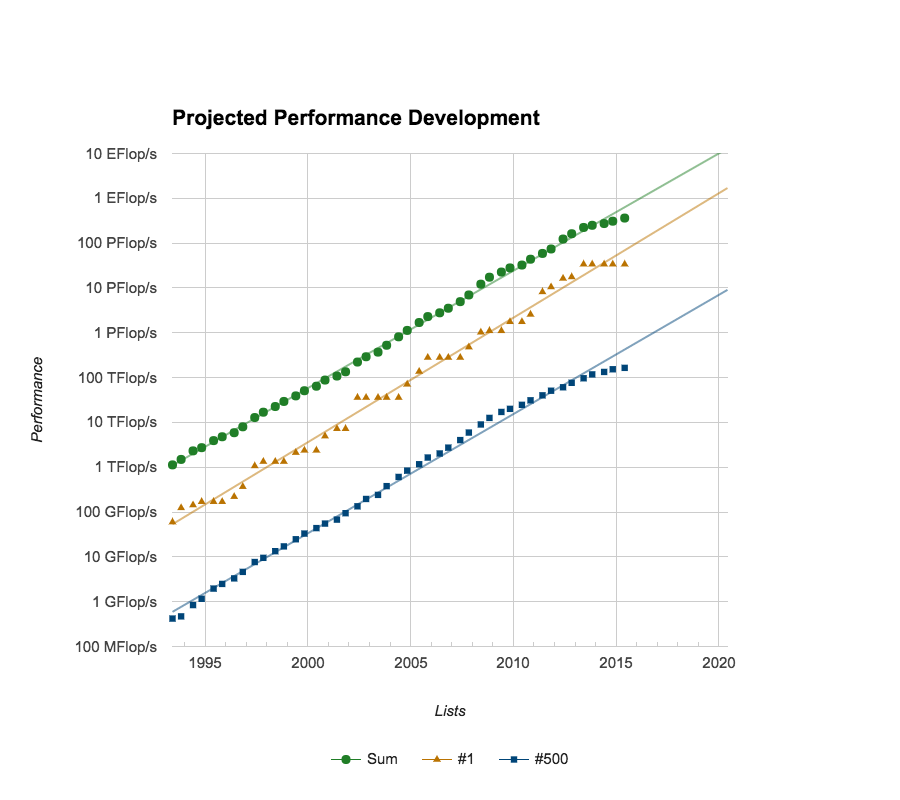
\includegraphics[width=0.95\textwidth]{./top500}
    \end{columns}
  \end{itemize}
\end{frame}

\begin{frame}
  \frametitle{  }
  \begin{itemize}
  \item Consider an example of moving a pile of boxes from location A to location B
  \item Lets say, it takes x mins per box. Total time required to move the boxes is 25x.
  \item How do you speed up moving 25 boxes from Location A to Location B?
  \end{itemize}
  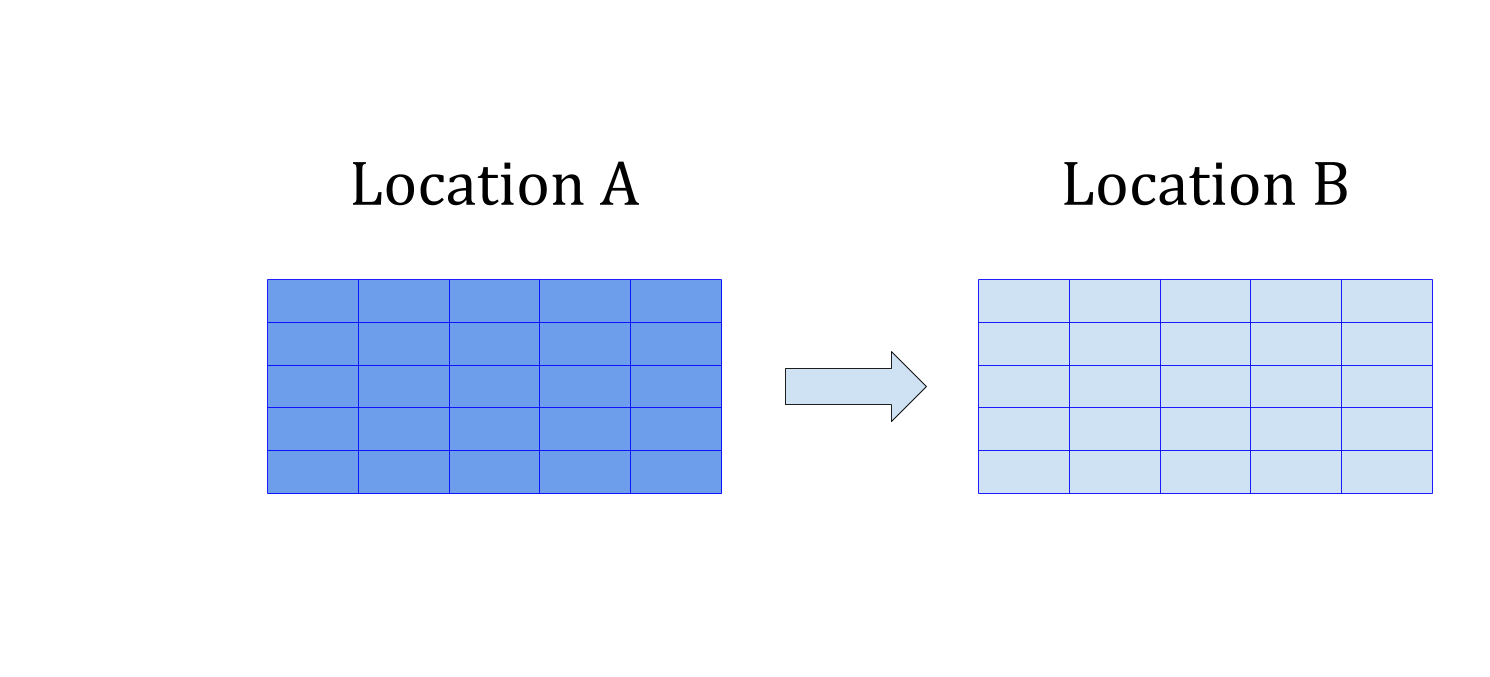
\includegraphics[width=\textwidth,clip=true]{./Serial}
\end{frame}

\begin{frame}
  \frametitle{ }
  \begin{itemize}
  \item You enlist more people to move the boxes.
  \item If 5 people move the boxes simultaneously, it should theoretically take 5x mins to move 25 boxes.
  \end{itemize}
  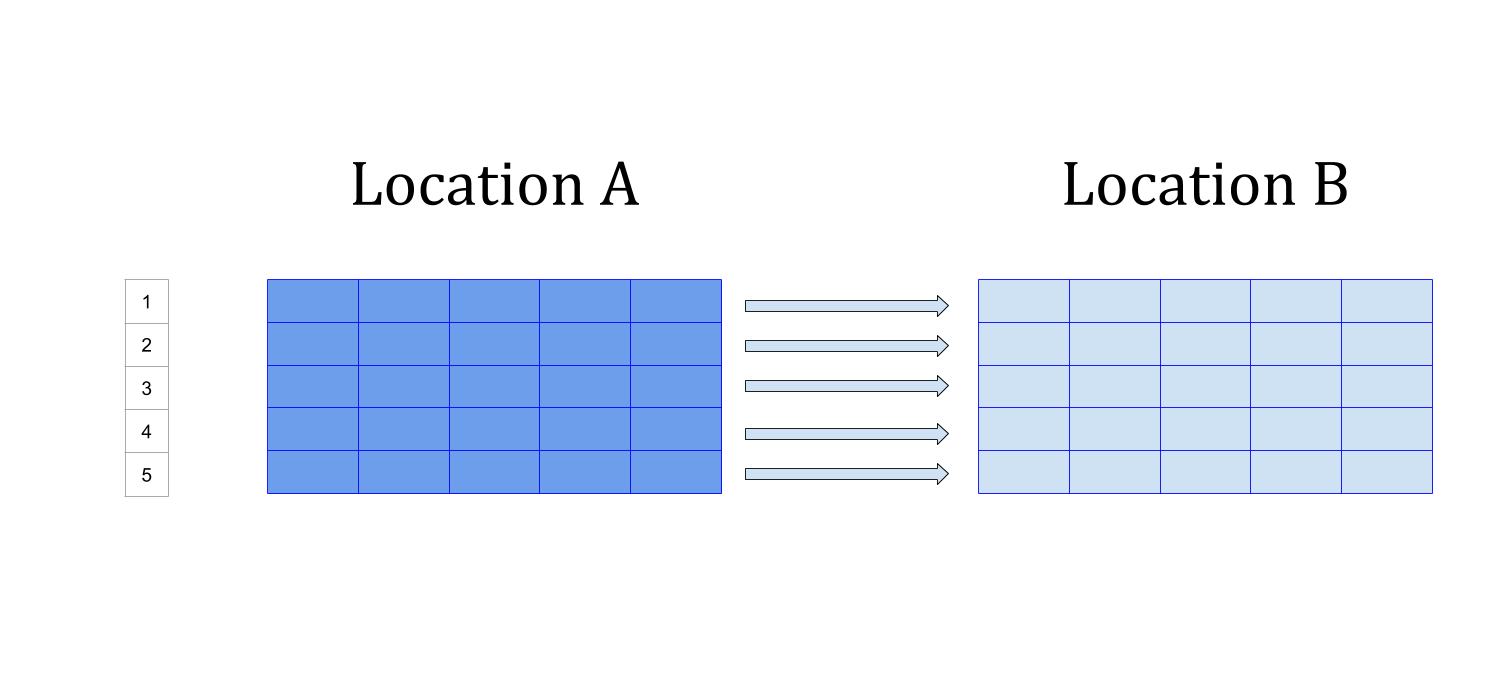
\includegraphics[width=\textwidth,clip=true]{./Parallel}
\end{frame}

\begin{frame}
  \frametitle{Evaluating Parallel Programs}
  \begin{itemize}
  \item Speedup
    \begin{itemize}
    \item Let $N_{\mathrm{Proc}}$ be the number of parallel processes
    \item[] 
    \item $\mathrm{Speedup}(N_{\mathrm{Proc}}) = \dfrac{\mathrm{Time\,used\,by\,best\,serial\,program}}{\mathrm{Time\,used\,by\,parallel\,program}}$ 
    \item[]
    \item Speedup is usually between 0 and $N_{\mathrm{Proc}}$
    \item[] 
    \end{itemize}
  \item Efficiency
    \begin{itemize}
    \item[]
    \item $\mathrm{Efficiency}(N_{\mathrm{Proc}}) = \dfrac{\mathrm{Speedup}(N_{\mathrm{Proc}})}{N_{\mathrm{Proc}}}$
    \item[]
    \item Efficiency is usually between 0 and 1
    \end{itemize}
  \end{itemize}
\end{frame}

\begin{frame}
  \frametitle{Speedup as a function of $N_{\mathrm{Proc}}$}
  \begin{columns}[c]
    \column{0.5\textwidth}
    \begin{itemize}
    \item Ideally
      \begin{itemize}
      \item The speedup will be linear
      \end{itemize}
    \item Even better
      \begin{itemize}
      \item (in very rare cases) we can have superlinear speedup
      \end{itemize}
    \item But in reality
      \begin{itemize}
      \item Efficiency decreases with increasing number of processes
      \end{itemize}
    \end{itemize}
    \column{0.5\textwidth}
    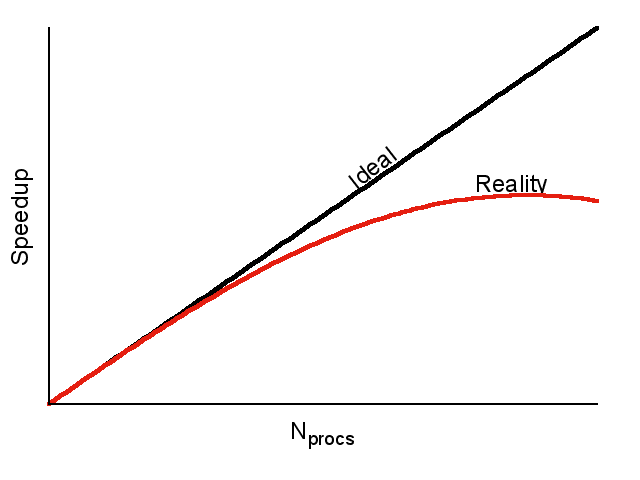
\includegraphics[width=\textwidth]{./speedup}
%    \begin{tikzpicture}[domain=0:1.8,scale=2]
%      %    \draw[very thin,color=gray] (0.0,0.0) grid (2.0,2.0);
%      \draw[->] (0,0) -- (2.0,0) node[below] {$N_{\mathrm{Proc}}$};
%      \draw[->] (0,0) -- (0,2.0) node[above] {Speedup};
%      \draw[color=red] plot[id=x] function{x} 
%      node[above] {Ideal};
%      \draw[color=blue] plot[id=sin] function{sin(x)} 
%      node[above] {Reality};
%    \end{tikzpicture}
  \end{columns}
\end{frame}

\begin{frame}
  \frametitle{Amdahl's Law}
  \begin{itemize}
  \item Let $f$ be the fraction of the serial program that cannot be parallelized
  \item Assume that the rest of the serial program can be perfectly parallelized (linear speedup)
    \begin{gather*}
      \mathrm{Time}_\mathrm{parallel} = \mathrm{Time}_\mathrm{serial}\cdot\left(f +\frac{1-f}{N_\mathrm{proc}}\right)
    \end{gather*}
  \item Or
    \begin{gather*}
      \mathrm{Speedup} = \cfrac{1}{f+\cfrac{1-f}{N_\mathrm{proc}}}\le\frac{1}{f}
    \end{gather*}
  \end{itemize}
\end{frame}

\begin{frame}{Maximal Possible Speedup}
  \begin{center}
    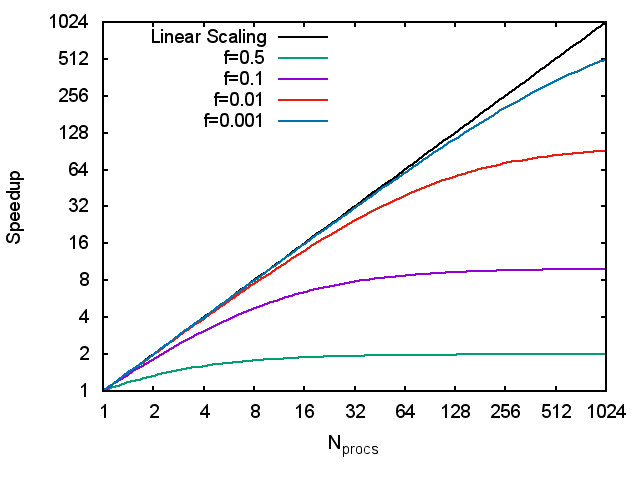
\includegraphics[width=0.9\textwidth]{./amdahl}
  \end{center}
\end{frame}

\begin{frame}
  \frametitle{Amdahl's Law}
  \begin{itemize}
  \item What Amdahl's law says
    \begin{itemize}
    \item It puts an upper bound on speedup (for a given $f$), no matter how many processes are thrown at it
    \end{itemize}
  \item Beyond Amdahl's law
    \begin{itemize}
    \item Parallelization adds overhead (communication)
    \item $f$ could be a variable too
      \begin{itemize}
      \item It may drop when problem size and $N_\mathrm{proc}$ increase
      \end{itemize}
    \item Parallel algorithm is different from the serial one
    \end{itemize}
  \end{itemize}
\end{frame}

\begin{frame}
  \frametitle{Writing a parallel program step by step}
  \begin{enumerate}
  \item Start from serial programs as a baseline
    \begin{itemize}
    \item Something to check correctness and efficiency against
    \end{itemize}
  \item Analyze and profile the serial program
    \begin{itemize}
    \item Identify the "hotspot"
    \item Identify the parts that can be parallelized
    \end{itemize}
  \item Parallelize code incrementally
  \item Check correctness of the parallel code
  \item Iterate step 3 and 4
  \end{enumerate}
\end{frame}


\begin{frame}
  \frametitle{A REAL example of parallel computing}
  \begin{itemize}
  \item Dense matrix multiplication $M_{md}\times{}N_{dn}=P_{mn}$
  \end{itemize}
  \begin{align*}
    P_{m,n} &= \sum_{k=1}^{d}M_{m,k}\times{}N_{k,n}\\
    P_{2,2} &= M_{2,1}*N_{1,2}+M_{2,2}*N_{2,2}+M_{2,3}*N_{3,2}+M_{2,4}*N_{4,2}
  \end{align*}
  \begin{center}
    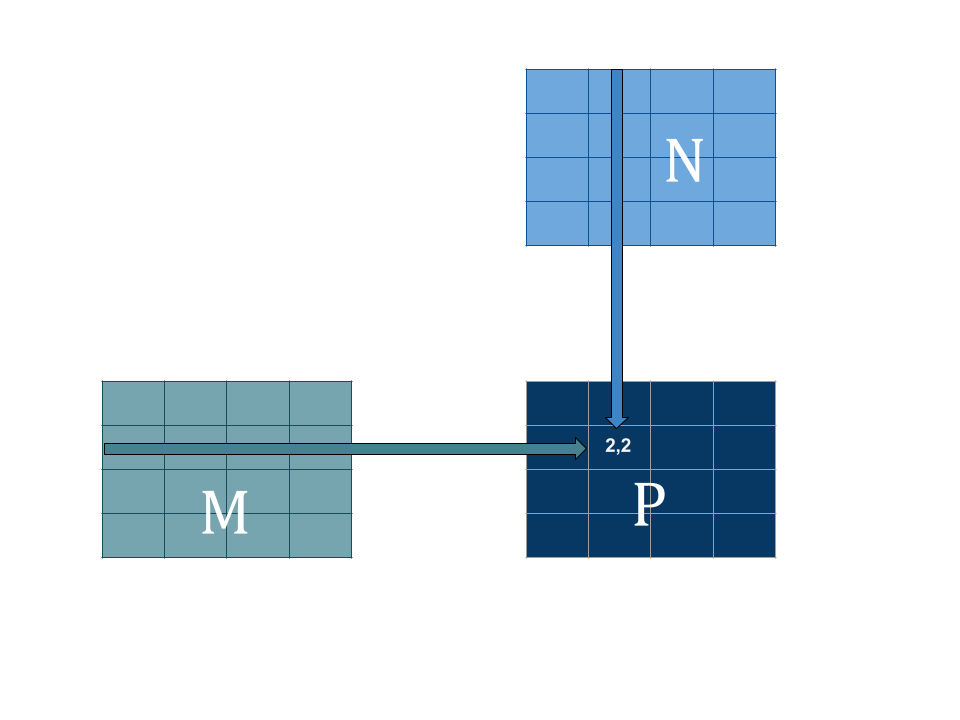
\includegraphics[width=0.7\textwidth]{./MatMul}
  \end{center}
\end{frame}

\begin{frame}
  \frametitle{Parallelizing matrix multiplication}
  \begin{itemize}
  \item Divide work among processors
  \item In our 4x4 example
    \begin{itemize}
    \item Assuming 4 processors
    \item Each responsible for a 2x2 tile (submatrix)
    \item Can we do 4x1 or 1x4?
    \end{itemize}
  \end{itemize}
  \begin{center}
    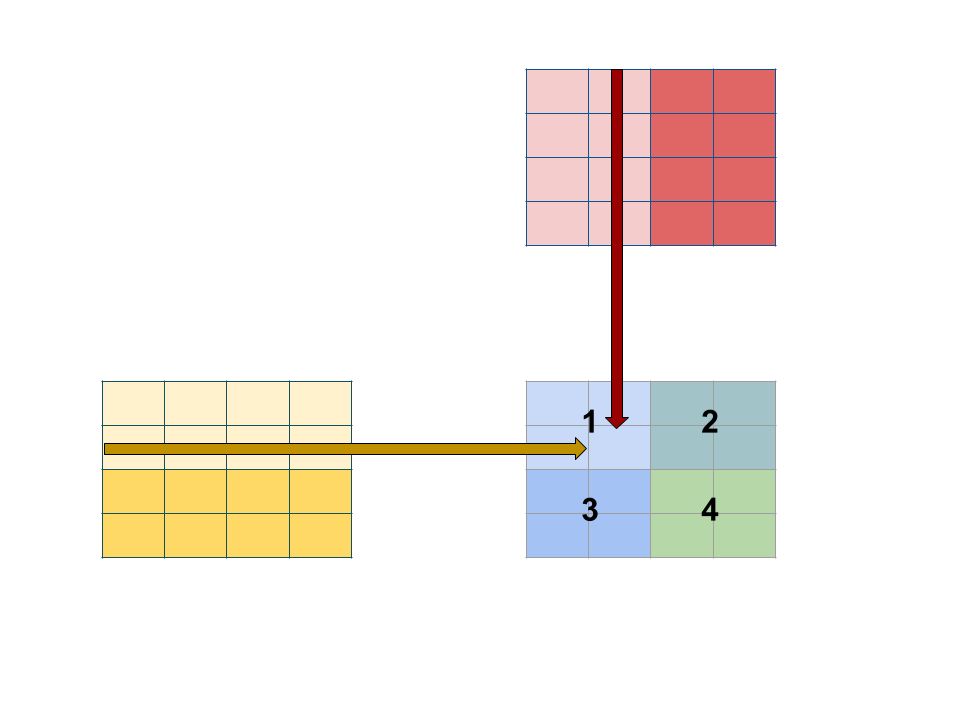
\includegraphics[width=0.7\textwidth]{./ParMatMul}
  \end{center}
\end{frame}

\begin{frame}[fragile]
  \frametitle{Pseudo Code}
  \begin{columns}
    \column{0.46\textwidth}
    \begin{exampleblock}{Serial}
      \begin{lstlisting}[language=C]
for i = 1, 4
  for j = 1, 4
    for k = 1, 4
       P(i,j) += M(i,k)*N(k,j);
      \end{lstlisting}
    \end{exampleblock}
    \column{0.46\textwidth}
    \begin{exampleblock}{Parallel}
      \begin{lstlisting}[language=C]
for i = istart, iend
  for j = jstart, jend
    for k = 1, 4
       P(i,j) += M(i,k)*N(k,j);
      \end{lstlisting}
    \end{exampleblock}
  \end{columns}
\end{frame}

\section{Parallel programming models}
\begin{frame}
  \frametitle{Single Program Multiple Data (SPMD)}
  \begin{itemize}
  \item All program instances execute same program
  \item Data parallel - Each instance works on different part of the data
  \item The majority of parallel programs are of this type
  \item Can also have
    \begin{itemize}
    \item SPSD: serial program
    \item MPSD: rare
    \item MPMD 
    \end{itemize}
  \end{itemize}
\end{frame}

\begin{frame}
  \frametitle{Memory system models}
  \begin{itemize}
  \item Different ways of sharing data among processors
    \begin{itemize}
    \item Distributed Memory
    \item Shared Memory
    \item Other memory models
      \begin{itemize}
      \item Hybrid model
      \item PGAS (Partitioned Global Address Space) 
      \end{itemize}
    \end{itemize}
  \end{itemize}
\end{frame}

\begin{frame}
  \frametitle{Distributed Memory Model}
  \begin{itemize}
  \item Each process has its own address space
    \begin{itemize}
    \item Data is local to each process
    \end{itemize}
  \item Data sharing is achieved via explicit message passing
  \item Example
    \begin{itemize}
    \item MPI
    \end{itemize}
  \end{itemize}
  \begin{center}
      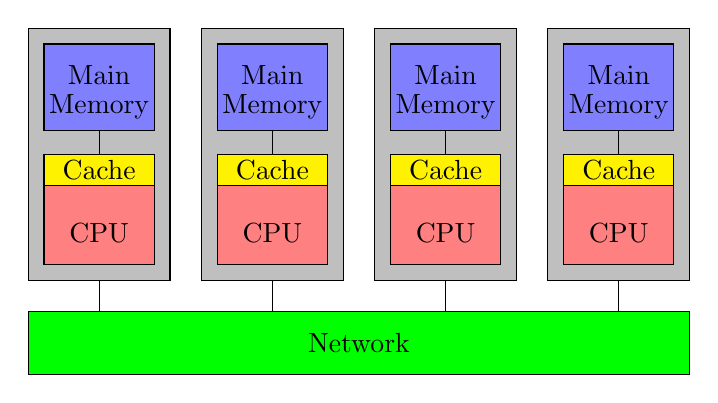
\begin{tikzpicture}[scale=0.4]
        \filldraw[fill=green] (0,-1) rectangle (21,-3);
        \draw (10.5,-2.0) node {Network};
        % First Node
        \filldraw[fill=gray!50!white] (0,0) rectangle (4.5,8);
        \filldraw[fill=blue!50!white] (0.5,4.75) rectangle (4.0,7.5);
        \filldraw[fill=yellow] (0.5,3.0) rectangle (4.0,4,0);
        \filldraw[fill=red!50!white] (0.5,0.5) rectangle (4.0,3.0);
        \draw (2.25,4.0) -- (2.25,4.75);
        \draw (2.25,0) -- (2.25,-1);
        \draw (2.25,6.5) node {Main};
        \draw (2.25,5.5) node {Memory};
        \draw (2.25,1.5) node {CPU};
        \draw (2.25,3.5) node {Cache};
        
        % Second Node
        \filldraw[fill=gray!50!white] (5.5,0) rectangle (10.0,8);
        \filldraw[fill=blue!50!white] (6.0,4.75) rectangle (9.5,7.5);
        \filldraw[fill=yellow] (6.0,3.0) rectangle (9.5,4,0);
        \filldraw[fill=red!50!white] (6.0,0.5) rectangle (9.5,3.0);
        \draw (7.75,4.0) -- (7.75,4.75);
        \draw (7.75,0) -- (7.75,-1);
        \draw (7.75,6.5) node {Main};
        \draw (7.75,5.5) node {Memory};
        \draw (7.75,1.5) node {CPU};
        \draw (7.75,3.5) node {Cache};
        
        % Third Node
        \filldraw[fill=gray!50!white] (11.0,0) rectangle (15.5,8);
        \filldraw[fill=blue!50!white] (11.5,4.75) rectangle (15.0,7.5);
        \filldraw[fill=yellow] (11.5,3.0) rectangle (15.0,4,0);
        \filldraw[fill=red!50!white] (11.5,0.5) rectangle (15.0,3.0);
        \draw (13.25,4.0) -- (13.25,4.75);
        \draw (13.25,0) -- (13.25,-1);
        \draw (13.25,6.5) node {Main};
        \draw (13.25,5.5) node {Memory};
        \draw (13.25,1.5) node {CPU};
        \draw (13.25,3.5) node {Cache};
        
        % Fourth Node
        \filldraw[fill=gray!50!white] (16.5,0) rectangle (21.0,8);
        \filldraw[fill=blue!50!white] (17.0,4.75) rectangle (20.5,7.5);
        \filldraw[fill=yellow] (17.0,3.0) rectangle (20.5,4,0);
        \filldraw[fill=red!50!white] (17.0,0.5) rectangle (20.5,3.0);
        \draw (18.75,4.0) -- (18.75,4.75);
        \draw (18.75,0) -- (18.75,-1);
        \draw (18.75,6.5) node {Main};
        \draw (18.75,5.5) node {Memory};
        \draw (18.75,1.5) node {CPU};
        \draw (18.75,3.5) node {Cache};
      \end{tikzpicture}
    \end{center}
\end{frame}

\begin{frame}
  \frametitle{Shared Memory Model}
  \begin{itemize}
  \item All threads can access the global memory space.
  \item Data sharing achieved via writing to/reading from the same memory location
  \item Example
    \begin{itemize}
    \item OpenMP
    \item Pthreads
    \end{itemize}
  \end{itemize}
  \begin{center}
      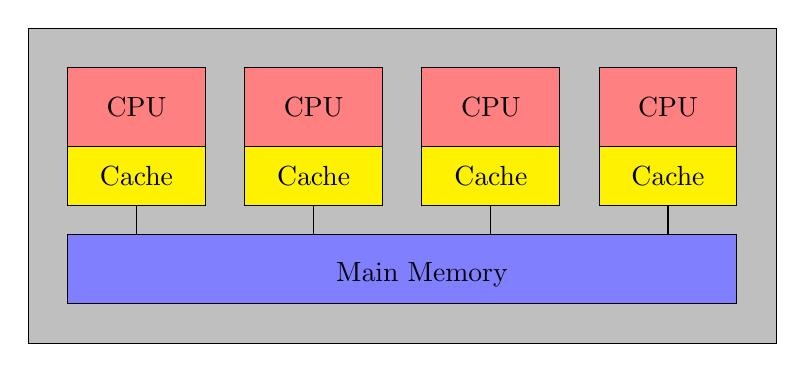
\begin{tikzpicture}[scale=0.5]
        \filldraw[fill=gray!50!white] (0,0) rectangle (19,8);
        \filldraw[fill=blue!50!white] (1,1) rectangle (18,2.75);
        \draw (10,1.75) node {Main Memory};
        % First Core
        \filldraw[fill=yellow] (1,3.5) rectangle (4.5,5.0);
        \draw (2.75,4.25) node {Cache};
        \filldraw[fill=red!50!white] (1,5.0) rectangle (4.5,7.0);
        \draw (2.75,6.0) node {CPU};
        \draw (2.75,3.5) -- (2.75,2.75);
        % Second Core
        \filldraw[fill=yellow] (5.5,3.5) rectangle (9.0,5.0);
        \draw (7.25,4.25) node {Cache};
        \filldraw[fill=red!50!white] (5.5,5.0) rectangle (9.0,7.0);
        \draw (7.25,6.0) node {CPU};
        \draw (7.25,3.5) -- (7.25,2.75);
        % Third Core
        \filldraw[fill=yellow] (10.0,3.5) rectangle (13.5,5.0);
        \draw (11.75,4.25) node {Cache};
        \filldraw[fill=red!50!white] (10.0,5.0) rectangle (13.5,7.0);
        \draw (11.75,6.0) node {CPU};
        \draw (11.75,3.5) -- (11.75,2.75);
        % Fourth Core
        \filldraw[fill=yellow] (14.5,3.5) rectangle (18.0,5.0);
        \draw (16.25,4.25) node {Cache};
        \filldraw[fill=red!50!white] (14.5,5.0) rectangle (18.0,7.0);
        \draw (16.25,6.0) node {CPU};
        \draw (16.25,3.5) -- (16.25,2.75);
      \end{tikzpicture}
%      \includegraphics[width=8cm]{./shared}
    \end{center}
\end{frame}

\begin{frame}
  \frametitle{Shared vs Distributed}
  \begin{columns}
    \column{5cm}
    \begin{description}
    \item {Shared}
    \end{description}
    \begin{itemize}
    \item Pros
      \begin{itemize}
      \item Global address space is user friendly
      \item Data sharing is fast
      \end{itemize}
    \item Cons
      \begin{itemize}
      \item Lack of scalability
      \item Data conflict issues
      \end{itemize}
    \end{itemize}
    \column{5cm}
    \begin{description}
    \item {Distributed}
    \end{description}
    \begin{itemize}
    \item Pros
      \begin{itemize}
      \item Memory scalable with number of processors
      \item Easier and cheaper to build
      \end{itemize}
    \item Cons
      \begin{itemize}
      \item Difficult load balancing
      \item Data sharing is slow
      \end{itemize}
    \end{itemize}
  \end{columns}
\end{frame}

\begin{frame}
  \frametitle{Hybrid model}
  \begin{itemize}
  \item Clusters of SMP (symmetric multi-processing) nodes dominate nowadays
  \item Hybrid model matches the physical structure of SMP clusters
    \begin{itemize}
    \item OpenMP within nodes
    \item MPI between nodes
    \end{itemize}
    \begin{center}
    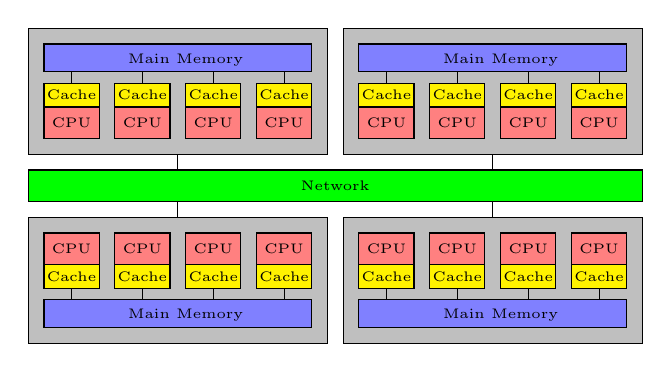
\begin{tikzpicture}[scale=0.2]
      \tikzstyle{every node}=[font=\tiny]
      \filldraw[fill=green] (0,9) rectangle (39,11);
      \draw (19.5,10) node {Network};
      % First Node
      \filldraw[fill=gray!50!white] (0,0) rectangle (19,8);
      \filldraw[fill=blue!50!white] (1,1) rectangle (18,2.75);
      \draw (10,1.75) node {Main Memory};
      % First Core
      \filldraw[fill=yellow] (1,3.5) rectangle (4.5,5.0);
      \draw (2.75,4.25) node {Cache};
      \filldraw[fill=red!50!white] (1,5.0) rectangle (4.5,7.0);
      \draw (2.75,6.0) node {CPU};
      \draw (2.75,3.5) -- (2.75,2.75);
      % Second Core
      \filldraw[fill=yellow] (5.5,3.5) rectangle (9.0,5.0);
      \draw (7.25,4.25) node {Cache};
      \filldraw[fill=red!50!white] (5.5,5.0) rectangle (9.0,7.0);
      \draw (7.25,6.0) node {CPU};
      \draw (7.25,3.5) -- (7.25,2.75);
      % Third Core
      \filldraw[fill=yellow] (10.0,3.5) rectangle (13.5,5.0);
      \draw (11.75,4.25) node {Cache};
      \filldraw[fill=red!50!white] (10.0,5.0) rectangle (13.5,7.0);
      \draw (11.75,6.0) node {CPU};
      \draw (11.75,3.5) -- (11.75,2.75);
      % Fourth Core
      \filldraw[fill=yellow] (14.5,3.5) rectangle (18.0,5.0);
      \draw (16.25,4.25) node {Cache};
      \filldraw[fill=red!50!white] (14.5,5.0) rectangle (18.0,7.0);
      \draw (16.25,6.0) node {CPU};
      \draw (16.25,3.5) -- (16.25,2.75);
      % Connect First Node to Network
      \draw (9.5,8) -- (9.5,9);

      % Second Node
      \filldraw[fill=gray!50!white] (20,0) rectangle (39,8);
      \filldraw[fill=blue!50!white] (21,1) rectangle (38,2.75);
      \draw (30,1.75) node {Main Memory};
      % First Core
      \filldraw[fill=yellow] (21,3.5) rectangle (24.5,5.0);
      \draw (22.75,4.25) node {Cache};
      \filldraw[fill=red!50!white] (21,5.0) rectangle (24.5,7.0);
      \draw (22.75,6.0) node {CPU};
      \draw (22.75,3.5) -- (22.75,2.75);
      % Second Core
      \filldraw[fill=yellow] (25.5,3.5) rectangle (29.0,5.0);
      \draw (27.25,4.25) node {Cache};
      \filldraw[fill=red!50!white] (25.5,5.0) rectangle (29.0,7.0);
      \draw (27.25,6.0) node {CPU};
      \draw (27.25,3.5) -- (27.25,2.75);
      % Third Core
      \filldraw[fill=yellow] (30.0,3.5) rectangle (33.5,5.0);
      \draw (31.75,4.25) node {Cache};
      \filldraw[fill=red!50!white] (30.0,5.0) rectangle (33.5,7.0);
      \draw (31.75,6.0) node {CPU};
      \draw (31.75,3.5) -- (31.75,2.75);
      % Fourth Core
      \filldraw[fill=yellow] (34.5,3.5) rectangle (38.0,5.0);
      \draw (36.25,4.25) node {Cache};
      \filldraw[fill=red!50!white] (34.5,5.0) rectangle (38.0,7.0);
      \draw (36.25,6.0) node {CPU};
      \draw (36.25,3.5) -- (36.25,2.75);
      % Connect Second Node to Network
      \draw (29.5,8) -- (29.5,9);

      % Third Node
      \filldraw[fill=gray!50!white] (0,12) rectangle (19,20);
      \filldraw[fill=blue!50!white] (1,17.25) rectangle (18,19);
      \draw (10,18.0) node {Main Memory};
      % First Core
      \filldraw[fill=yellow] (1,16.5) rectangle (4.5,15.0);
      \draw (2.75,15.75) node {Cache};
      \filldraw[fill=red!50!white] (1,15.0) rectangle (4.5,13.0);
      \draw (2.75,14.0) node {CPU};
      \draw (2.75,16.5) -- (2.75,17.25);
      % Second Core 
      \filldraw[fill=yellow] (5.5,16.5) rectangle (9.0,15.0);
      \draw (7.25,15.75) node {Cache};
      \filldraw[fill=red!50!white] (5.5,15.0) rectangle (9.0,13.0);
      \draw (7.25,14.0) node {CPU};
      \draw (7.25,16.5) -- (7.25,17.25);
      % Third Core 
      \filldraw[fill=yellow] (10.0,16.5) rectangle (13.5,15.0);
      \draw (11.75,15.75) node {Cache};
      \filldraw[fill=red!50!white] (10.0,15.0) rectangle (13.5,13.0);
      \draw (11.75,14.0) node {CPU};
      \draw (11.75,16.5) -- (11.75,17.25);
      % Fourth Core 
      \filldraw[fill=yellow] (14.5,16.5) rectangle (18.0,15.0);
      \draw (16.25,15.75) node {Cache};
      \filldraw[fill=red!50!white] (14.5,15.0) rectangle (18.0,13.0);
      \draw (16.25,14.0) node {CPU};
      \draw (16.25,16.5) -- (16.25,17.25);
      % Connect Third Node to Network
      \draw (9.5,11) -- (9.5,12);

      % Fourth Node
      \filldraw[fill=gray!50!white] (20,12) rectangle (39,20);
      \filldraw[fill=blue!50!white] (21,17.25) rectangle (38,19);
      \draw (30,18.0) node {Main Memory};
      % First Core
      \filldraw[fill=yellow] (21,16.5) rectangle (24.5,15.0);
      \draw (22.75,15.75) node {Cache};
      \filldraw[fill=red!50!white] (21,15.0) rectangle (24.5,13.0);
      \draw (22.75,14.0) node {CPU};
      \draw (22.75,16.5) -- (22.75,17.25);
      % Second Core 
      \filldraw[fill=yellow] (25.5,16.5) rectangle (29.0,15.0);
      \draw (27.25,15.75) node {Cache};
      \filldraw[fill=red!50!white] (25.5,15.0) rectangle (29.0,13.0);
      \draw (27.25,14.0) node {CPU};
      \draw (27.25,16.5) -- (27.25,17.25);
      % Third Core 
      \filldraw[fill=yellow] (30.0,16.5) rectangle (33.5,15.0);
      \draw (31.75,15.75) node {Cache};
      \filldraw[fill=red!50!white] (30.0,15.0) rectangle (33.5,13.0);
      \draw (31.75,14.0) node {CPU};
      \draw (31.75,16.5) -- (31.75,17.25);
      % Fourth Core 
      \filldraw[fill=yellow] (34.5,16.5) rectangle (38.0,15.0);
      \draw (36.25,15.75) node {Cache};
      \filldraw[fill=red!50!white] (34.5,15.0) rectangle (38.0,13.0);
      \draw (36.25,14.0) node {CPU};
      \draw (36.25,16.5) -- (36.25,17.25);
      % Connect Fourth Node to Network
      \draw (29.5,11) -- (29.5,12);
      
    \end{tikzpicture}
  \end{center}
  \end{itemize}
\end{frame}

\begin{frame}
  \frametitle{Potential benefits of hybrid model}
  \begin{itemize}
  \item Message-passing within nodes (loopback) is eliminated
  \item Number of MPI processes is reduced, which means
    \begin{itemize}
    \item Message size increases
    \item Message number decreases
    \end{itemize}
  \item Memory usage could be reduced
    \begin{itemize}
    \item Eliminate replicated data
    \end{itemize}
  \item Those are good, but in reality, (most) pure MPI programs run as fast (sometimes faster than) as hybrid
    ones $\cdots$
  \end{itemize}
\end{frame}

\begin{frame}
  \frametitle{Reasons why NOT to use hybrid model}
  \begin{itemize}
  \item Some (most?) MPI libraries already use internally different protocols
    \begin{itemize}
    \item Shared memory data exchange within SMP nodes
    \item Network communication between SMP nodes
    \end{itemize}
  \item Overhead associated with thread management
    \begin{itemize}
    \item Thread fork/join
    \item Additional synchronization with hybrid programs 
    \end{itemize}
  \end{itemize}
\end{frame}

\section{Parallel programming hurdles}
\begin{frame}
  \frametitle{Parallel Programming Hurdles}
  \begin{itemize}
  \item Hidden serializations
  \item Overhead caused by parallelization
  \item Load balancing
  \item Synchronization issues
  \end{itemize}
\end{frame}

\begin{frame}
  \frametitle{Hidden Serialization}
  \begin{itemize}
  \item Back to our box moving example
  \item What if there is a very long corridor that allows only one work to pass at a time between Location A and B?
  \end{itemize}
  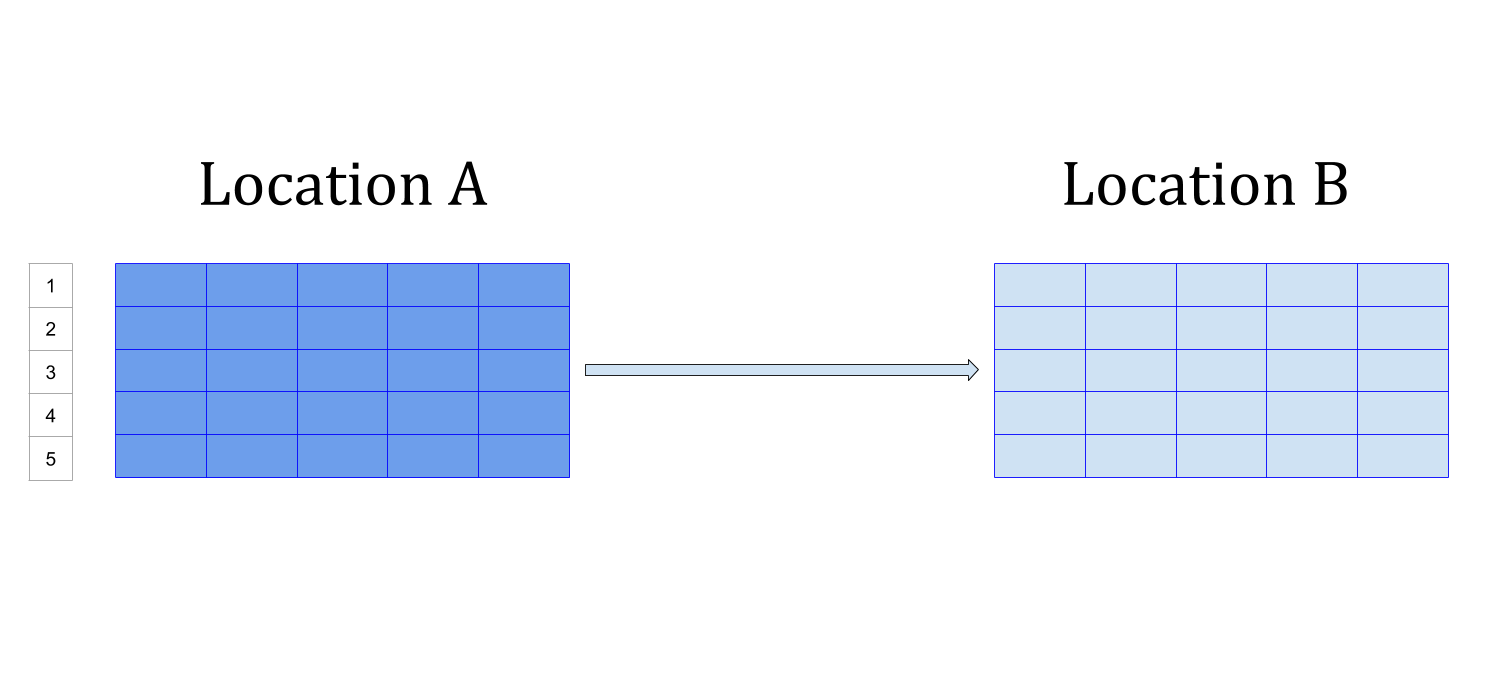
\includegraphics[width=\textwidth]{./Parallel_Load}
\end{frame}

\begin{frame}
  \frametitle{Hidden Serialization}
  \begin{itemize}
  \item It is not the part in serial programs that is hard or impossible to parallelize
    \begin{itemize}
    \item Intrinsic serialization (the $f$ in Amdahl's law)
    \end{itemize}
  \item Examples of hidden serialization:
    \begin{itemize}
    \item System resources contention, e.g. I/O hotspot
    \item Internal serialization, e.g. library functions that cannot be executed in parallel for correctness
    \end{itemize}
  \end{itemize}
\end{frame}

\begin{frame}
  \frametitle{Communication overhead}
  \begin{itemize}
  \item Sharing data across network is slow
    \begin{itemize}
    \item Mainly a problem for distributed memory systems
    \end{itemize}
  \item There are two parts of it
    \begin{itemize}
    \item Latency: startup cost for each transfer
    \item Bandwidth: extra cost for each byte
    \end{itemize}
  \item Reduce communication overhead
    \begin{itemize}
    \item Avoid unnecessary message passing
    \item Reduce number of messages by combining them
    \end{itemize}
  \end{itemize}
\end{frame}

\begin{frame}
  \frametitle{Memory Heirarchy}
  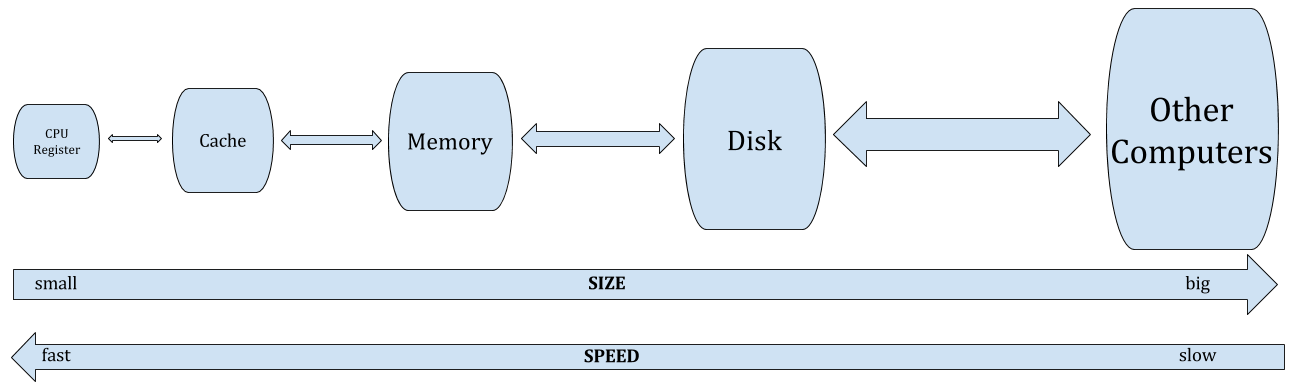
\includegraphics[width=\textwidth]{./MemHier}
  \begin{itemize}
  \item Avoid unnecessary data transfer
  \item Load data in blocks (spatial locality)
  \item Reuse loaded data (temporal locality)
  \item All these apply to serial programs as well
  \end{itemize}
\end{frame}

\begin{frame}
  \frametitle{Load balancing}
  \begin{itemize}
  \item Back to our box moving example, again
  \item Anyone sees a problem?
  \end{itemize}
  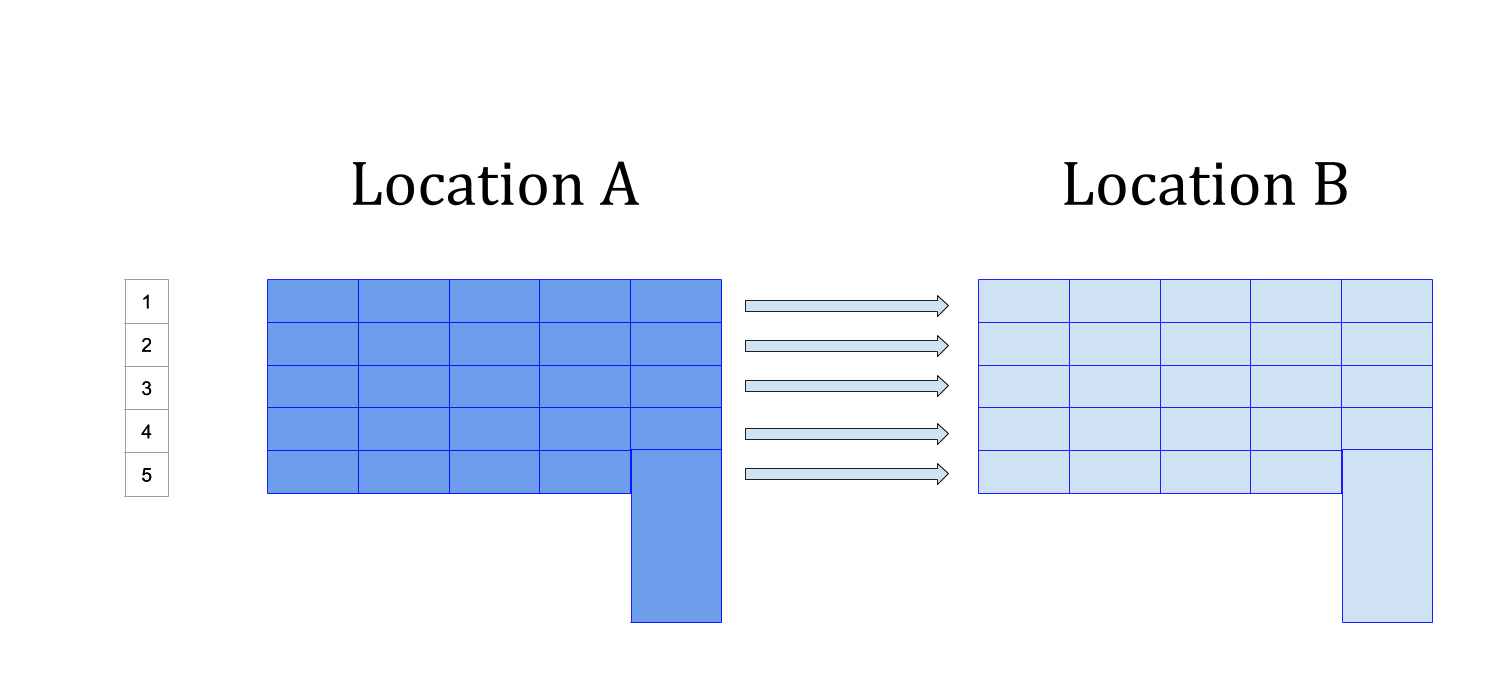
\includegraphics[width=\textwidth]{./Load-Balance}
\end{frame}

\begin{frame}
  \frametitle{Load balancing}
  \begin{itemize}
  \item Work load not evenly distributed
    \begin{itemize}
    \item Some are working while others are idle
    \item The slowest worker dominates in extreme cases
    \end{itemize}
  \item Solutions
    \begin{itemize}
    \item Explore various decomposition techniques
    \item Dynamic load balancing
    \end{itemize}
  \item Hard for distributed memory
  \item Adds overhead
  \end{itemize}
\end{frame}

\begin{frame}
  \frametitle{Synchronization issues - deadlock}
  \begin{center}
    
\includegraphics[width=0.5\textwidth]{./SBFP}
  \end{center}
\end{frame}

\begin{frame}
  \frametitle{Deadlock}
  \begin{itemize}
  \item Often caused by "blocking" communication operations
    \begin{itemize}
    \item "Blocking" means "I will not proceed until the current operation is over"
    \end{itemize}
  \item Solution
    \begin{itemize}
    \item Use "non-blocking" operations
    \item Caution: trade-off between data safety and performance
    \end{itemize}
  \end{itemize}
\end{frame}


\section{Heterogeneous computing}
\begin{frame}
  \frametitle{Heterogeneous computing}
  \begin{itemize}
  \item A heterogeneous system solves tasks using different types of processing units
    \begin{itemize}
    \item CPUs
    \item GPUs
    \item DSPs
    \item Co-processors
    \item $\cdots$
    \end{itemize}
  \item As opposed to homogeneous systems, e.g. SMP nodes with CPUs only
  \end{itemize}
\end{frame}

\begin{frame}
  \frametitle{The Free Lunch Is Over}
  \begin{center}
    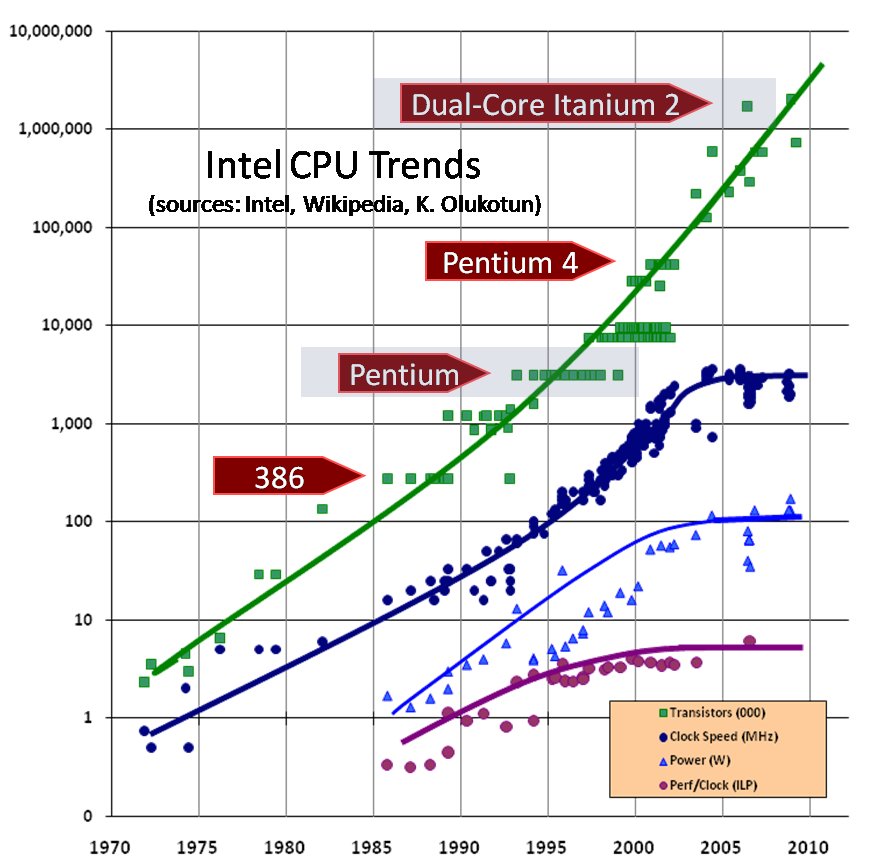
\includegraphics[width=0.6\textwidth]{CPUTrend}
    
    
    \tiny{Source: Herb Sutter\\
      http://www.gotw.ca/publications/concurrency-ddj.htm}
  \end{center}
\end{frame}

\begin{frame}
  \frametitle{Power and Clock Speed}
  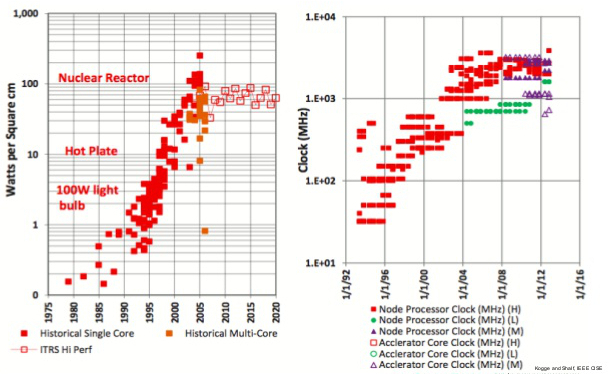
\includegraphics[width=\textwidth]{./CPUheat}
\end{frame}

\begin{frame}
  \frametitle{Power efficiency is the key}
  \begin{itemize}
  \item We have been able to make computer run faster by adding more transistors
    \begin{itemize}
    \item Moore's law
    \end{itemize}
  \item Unfortunately, not any more
    \begin{itemize}
    \item Power consumption/heat generation limits packing density
    \item $\mathrm{Power} \sim \mathrm{speed}^2$
    \end{itemize}
  \item Solution
    \begin{itemize}
    \item Reduce each core's speed and use more cores - increased
      parallelism
    \end{itemize}
  \end{itemize}
  \begin{center}
    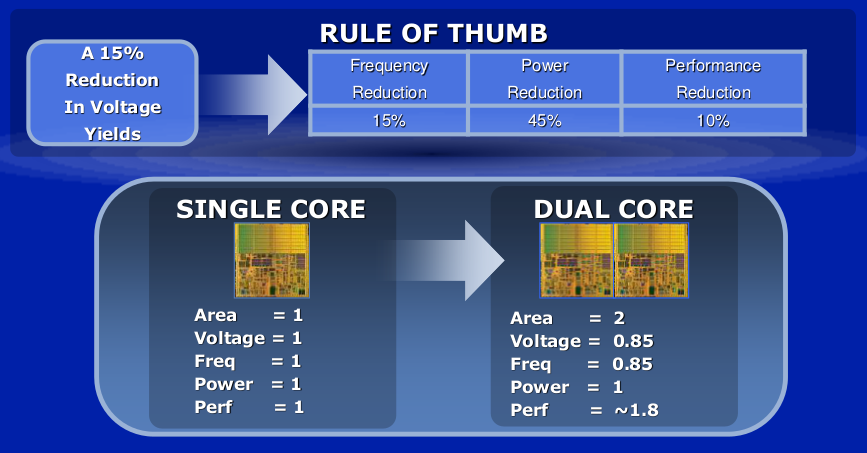
\includegraphics[width=0.6\textwidth]{./cpucore}
    
    \tiny{Source: John Urbanic, PSC}
  \end{center}
\end{frame}

\begin{frame}
  \frametitle{Graphic Processing Units (GPUs)}
  \begin{itemize}
  \item Massively parallel many-core architecture
    \begin{itemize}
    \item Thousands of cores capable of running millions of threads
    \item Data parallelism
    \end{itemize}
  \item GPUs are traditionally dedicated for graphic rendering, but
    become more versatile thanks to
    \begin{itemize}
    \item Hardware: faster data transfer and more on-board memory
    \item Software: libraries that provide more general purposed
      functions
    \end{itemize}
  \item GPU vs CPU
    \begin{itemize}
    \item GPUs are very effectively for certain type of tasks, but we still need the general purpose CPUs
    \end{itemize}
  \end{itemize}
\end{frame}
\begin{frame}
  \frametitle{nVIDIA Kepler K80}
  \begin{columns}[c]
    \column{0.5\textwidth}
    \begin{itemize}
    \item Performance: 
      \begin{itemize}
      \item 1.87 TFlops (DP)
      \item 5.6 TFlops (SP)
      \end{itemize}
    \item GPU: 2x GK210
    \item CUDA Cores: 4992
    \item Memory (GDDR5): 24GB
    \item Memory (Bandwidth): 480GBs
    \item Features
      \begin{itemize}
      \item 192 SP CUDA Cores
      \item 64 DP units
      \item 32 Special function units (SFU)
      \item 32 load/store units (LD/ST)
      \end{itemize}
    \end{itemize}
    \column{0.5\textwidth}
    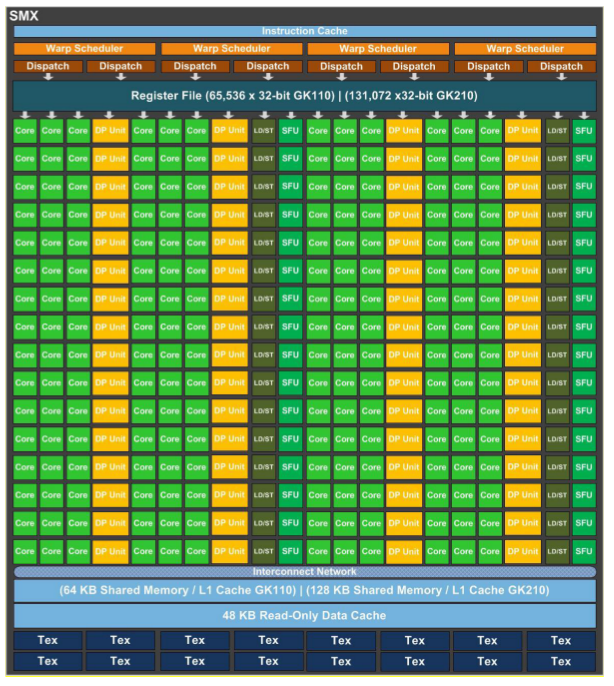
\includegraphics[width=\textwidth]{./GK210-110}
  \end{columns}
\end{frame}

\begin{frame}
  \frametitle{GPU programming strategies}
  \begin{itemize}
  \item GPUs need to copy data from main memory to its onboard
    memory and copy them back
    \begin{itemize}
    \item Data transfer over PCIe is the bottleneck, so one needs to
    \end{itemize}
  \item Avoid data transfer and reuse data
  \item Overlap data transfer and computation
  \item Massively parallel, so it is a crime to do anything antiparallel
    \begin{itemize}
    \item Need to launch enough threads in parallel to keep the
      device busy
    \item Threads need to access contiguous data
    \item Thread divergence needs to be eliminated
    \end{itemize}
  \end{itemize}
\end{frame}

\begin{frame}
  \frametitle{Intel Many Integrated Core Architecture}
  \begin{itemize}
  \item Leverage x86 architecture (CPU with many cores)
  \item[] X86 cores are simpler, but allow for more compute throughput
  \item Leverage existing x86 programming models
  \item Dedicate much of the silicon to floating point ops
  \item Cache coherent
  \item Increase floating-point throughput
  \item Implement as a separate device
  \item Strip expensive features (out-of-order execution, branch prediction,
    etc.)
  \item Widen SIMD registers for more throughput
  \item Fast (GDDR5) memory on card
  \item Runs a full Linux operating system (BusyBox)
  \end{itemize}
\end{frame}

\begin{frame}
  \frametitle{Intel Xeon Phi 7120P}
  \begin{itemize}
  \item Add-on to CPU-based system
  \item 16 GB memory
  \item 61 x86 64-bit cores (244 threads)
  \item single-core 1.2 GHz
  \item 512-bit vector registers
  \item 1.208 TFLOPS = 61 cores * 1.238 GHz * 16 DP FLOPs/cycle/core
  \end{itemize}
  \begin{center}
    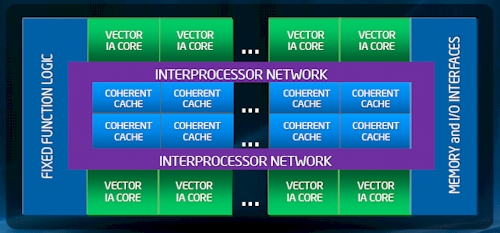
\includegraphics[width=0.75\textwidth]{./intel_hpc_mica}
  \end{center}
\end{frame}

\begin{frame}
  \frametitle{MICs comparison to GPUs}
  \begin{itemize}
  \item Disadvantages
    \begin{itemize}
    \item Less acceleration
    \item In terms of computing power, one GPU beats one Xeon Phi
      for most cases currently.
    \end{itemize}
  \item Advantages
    \begin{itemize}
    \item X86 architecture
    \item IP-addressable
    \item Traditional parallelization (OpenMP, MPI)
    \item Easy programming, minor changes from CPU codes
    \item Offload: minor change of source code.
    \item New. Still a lot of room for improvement.
    \end{itemize}
  \end{itemize}
\end{frame}

\end{document}
